\documentclass[a4paper, 12pt]{article}
%\usepackage[polish]{babel}
%\usepackage[cp1250]{inputenc}
\usepackage[latin2]{inputenc}
%\usepackage{polski}
\usepackage[T1]{fontenc}
\usepackage{graphicx}


\pagestyle{headings}
\textwidth      15.5cm
\oddsidemargin    .1cm
\evensidemargin   .1cm



\begin{document}

\thispagestyle{empty}

\begin{minipage}{5cm}
%
\includegraphics[scale=0.3]{logo.eps}
\end{minipage}
\begin{minipage}{10cm}
\begin{center}
{Salomon\\
System przetwarzania wiedzy\\}
\end{center}
\end{minipage}

\vspace*{0.5cm}

\hrulefill

\vspace*{1cm}


\begin{flushleft}

\section{Drzewa decyzyjne w teorii decyzji}

W teorii decyzji drzewo decyzyjne jest drzewem decyzji i ich mozliwych konsekwencji (stan�w natury). Zadaniem drzew decyzyjnych mo�e by� zar�wno stworzenie planu, jak i rozwiazanie problemu decyzyjnego.

Metoda drzew decyzyjnych jest szczeg�lnie przydatna w problemach decyzyjnych z licznymi, rozga�eziajacymi sie wariantami oraz w przypadku podejmowania decyzji w warunkach ryzyka.

\section{Drzewa decyzyjne w uczeniu maszynowym}

Drzewa decyzyjne w uczeniu maszynowym s�uzy do wyodrebniania wiedzy z zestawu przyk�ad�w (patrz eksploracja danych). Zak�adamy, ze posiadamy zestaw przyk�ad�w: obiekt�w opisanych przy pomocy atrybut�w, kt�rym przyporzadkowujemy jakas decyzje (patrz tabela decyzyjna).

Przyk�ad: Chcemy zautomatyzowa� proces przyjmowania kandydat�w na praktyki w duzej firmie. Posiadamy setki przyk�ad�w z przesz�osci, chcemy wydoby� z nich regu�y decyzyjne. Atrybuty Wykszta�cenie, Jezyki obce, Doswiadczenie i Og�lne wrazenie sa kodowane skala od 1 do 5.
\linebreak
%do poprawy
\begin{table}[h]
%\multicolumn{7}{c}{	}
Wiek 	P�e� 	Wykszta�cenie 	Jezyki 	Doswiadczenie 	Prezentacja 	Przyjety\linebreak 
25 	m 	2 	4 	1 	4 	nie\linebreak 
22 	k 	4 	3 	4 	2 	nie\linebreak 
21 	m 	4 	5 	5 	4 	tak\linebreak 
29 	m 	1 	3 	2 	3 	nie\linebreak 
\caption{}
\end{table} 
\linebreak
Na podstawie tabeli decyzyjnej tworzymy drzewo, kt�rego wez�ami sa poszczeg�lne atrybuty, ga�eziami wartosci odpowiadajace tym atrybutom, a liscie tworza poszczeg�lne decyzje. Na podstawie przyk�adowych danych wygenerowano nastepujace drzewo:



\begin{figure}
	\centering
	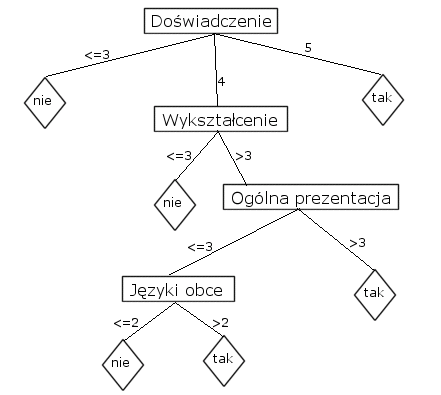
\includegraphics[bb=0 0 441 395]{Drzewo_decyzyjne.png}
% Drzewo_decyzyjne.png: 72dpi, width=15.56cm, height=13.93cm, bb=0 0 441 395
\end{figure}

Drzewo w takiej postaci odzwierciedla w jaki spos�b by�y na podstawie atrybut�w by�y podejmowane decyzje klasyfikujace (dla uproszczenia po�aczono niekt�re ga�ezie). Zaleta tej reprezentacji jest jej czytelnos� dla cz�owieka. W prosty spos�b mozna przekszta�ci� ja do reprezentacji regu�owej.

\section{Algorytm tworzenia drzewa ID3}
\subsection{W duzym skrocie}

Dopuki kazdy z lisci drzewa nie nalezy do tej samej klasy rownowaznosci (nie jest homogeniczny - jego zmienne decyzyjne nie sa jednakowe) powtarzaj:

    \begin{itemize}
\item Wybierz niehomogeniczny lisc
\item Zamien ten lisc na wezel testowy dzielacy ten podzbior na tak niehomogeniczne podzbiory jak to mozliwe, zgodnie z wyliczeniem entropii
\end{itemize}

\subsection{Troche dokladniej}
    \begin{itemize}
\item Oblicz entropie dla kazdego z atrybutow, ktore chcemy wykorzystac do tworzenia nastepnego poziomu drzewa
\ item Wybierz najlepszy z nich (ten ktory minimalizuje entropie)
\end{itemize}

\subsection{Minimalizacja entropii?}

Generalnie zalozenie jest aby tworzyc drzewa decyzyjne optymalnej wielkosci ale z praktycznego punktu widzenia nie jest to uzasadnione ze wzgledu na duzy koszt obliczeniowy. W zastepstwie korzystamy z przyblizonych procedur tworzenia malych, ale niekoniecznie najmniejszych drzew decyzyjnych.

\subsection{Wybieranie atrybutu do obliczania entropii}

Najwazniejszym punktem algorytmu ID3 jest wybor atrybutu do testowania na kazdym lisciu drzewa.

Procedura:
\begin{itemize}
\item Nalezy sprawdzic jak atrybut dzieli elementy nalezace do liscia
\item Minimalizuj srednia entropie (oblicz entropie dla kazdego z wezlow, dla kazdego z z atrybutow i wybierz ten z najmniejsza entropia
\end{itemize}

\subsection{Formula Entropii}

Entropia jest miara z teorii informacji, charakteryzujaca czystosc i homogenicznosc zbioru atrybutow. 

\subsubsection{Dane}
\begin{itemize}
\item nb, liczba instancji w lisciu b
\item nbc, liczba instancji w lisciu b nalezacych do klasy c. nbc <= nb
\item nt, calkowita liczna instancji we wszystkich lisciach
\end{itemize}

\subsubsection{Prawdopodobienstwo}
$P_{b}=\frac{n_{bc}}{n_{b}}$
\begin{itemize}
\item Jezeli wszystkie instancje w grupie sa klasyfikowane pozytywnie, wtedy Pb = 1 (lisc homogeniczny pozytywnie) 
\item Jezeli wszystkie instancje w grupie sa klasyfikowane negatywnie, wtedy Pb = 0 (lisc homogeniczny negatywnie) 
\end{itemize}


\subsubsection{Entropia}
$Entropia = Sum(c)(\frac{n_{bc}}{n_{b}})log_{2}(\frac{n_{bc}}{n_{b}})$

\begin{itemize}
\item Entropia jest zerowa jezeli zbior jest idealnie homogeniczny
\item Entropie wynosi 1 jezeli zbior jest idealnie niehomogeniczny ze wzgledu na atrybut (tzn. nie jest on dzielony na zadne podgrupy przez ten atrybut)
\end{itemize}

\subsubsection{Srednia entropia}
$Srednia entropia = Sum(b)(\frac{n_{b}}{n_{t}})*[Sum(c)(\frac{n_{bc}}{n_{b}})log_{2}(\frac{n_{bc}}{n_{b}})]$

\end{flushleft}
\end{document}
